%%AG: falta mencionar la figura 1 desde el texto
\begin{figure*}[h]
    \centering
    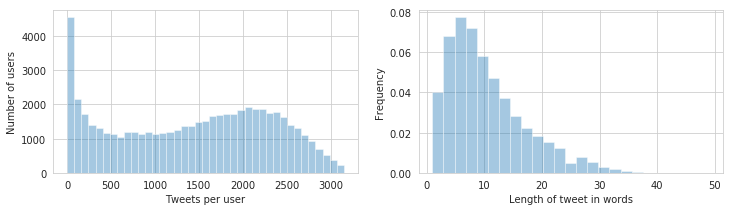
\includegraphics[width=\textwidth]{./images/dataset_histograms.png}
    \caption{Distributional figures of the dataset. Left: Distribution of number of tweets per user. Right: Distribution of length (in words) of tweets.} 
    \label{fig:tweets_distribution} 
 \end{figure*}

To gather our data, information of \textit{departments} in Argentina (the second-level administrative division of the country, after \textit{provinces}) was collected from the 2010 National Census.\footnote{\url{https://www.indec.gov.ar}} Next, a lookup was made through the Twitter API for users with location matching those departments, while balancing the number of users per province. The Python library \textit{tweepy} was used to interact with the Twitter API. 

Although we tried to retrieve users from every single department, we found that they concentrate mainly around larger cities. This phenomenon is due to limitations in the geographical information made available by Twitter. This is why we selected provinces as our geographical unit of study, rather than more fine-grained departments. We collected roughly 2400 users per province.

For these users, we retrieved their entire tweetlines. Tweets were tokenized using \emph{NLTK} \cite{bird2009natural}. Hashtags and mentions to users were removed; the remaining words were downcased; and identical consecutive vowels were normalized up to three repetitions (``woaaa'' instead of ``woaaaaaa''). Analogously to users, the number of words per province was also balanced. Table \ref{tab:summary_tweets} lists the figures for the collected dataset, and Figure \ref{fig:tweets_distribution} display the distributions of tweets per user and length of tweets.

\begin{table}[b]
\begin{center}

\begin{tabular}{lrrr}
            & Total   & Mean   & SD \\ % &           STD 
\hline 
Words       &  647M   &  28.14M & 6.64M  \\ %&  3.325680e+06 \\
Tweets      &  80.9M  &  3.51M  & 0.91M  \\ %&  4.571673e+05 \\
Users       &  56.2K  &  2.44K  & 0.04K  \\ %&  1.947665e+01 \\
Vocabulary  &   7.5M  &  0.32M  & 0.04M  \\ %&  2.619165e+04 \\
\hline
\end{tabular}


\caption{Dataset summary. Total figures are provided, along with province-level mean and standard deviation.}
\label{tab:summary_tweets}
\end{center}
\end{table}


It is well known that Twitter vocabulary tends to be very noisy \cite{kaufmann2010syntactic} with lots of contractions, non-normal spellings (e.g., vocalizations), typos, etc. Consequently, only words occurring more than 40 times and used by more than 25 users were taken into account. This removes about 1\% of the total words and reduces vocabulary from 2.3 million words to around 135 thousand words. 

While these preprocessing steps may seem insufficient for many linguistic analyses, we find them acceptable enough for our present study, given that the phenomenon of locally-used words will still be likely to emerge in spite of different spellings, typos and other morphological variations. Indeed, while the same word might appear with several variations or spellings, we expect at least one normalized form to be more frequent and thus stand out from the rest.







